\chapter{Methods and Results}
\label{methods} % Always give a unique label
%use \chaptermark{}
% to alter or adjust the chapter heading in the running head

\section{Force Measurement}
\label{sec:sysArch}

\begin{figure}[h]
	\begin{center}
		\includegraphics[width=100mm]{fig/methods/calib_setup.png}
	\end{center}
	\vspace{-4mm}
	\caption[Developed force-measuring system on the PSM]
	{Block diagram}
	\label{fig:PSM_with_FF}
	\vspace{-2mm}
\end{figure}

Block diagram of the created system for 3-DOF force measurement is shown on figure \ref{fig:BlockDiag}. Forces that applied on the end of surgical tool are measured using strain gauges, which change their resistance with force. Using created printed circuit boards (PCBs), this resistance changes are measured and published within ROS. At the same time we measure current joint position of the tool, which is needed for the force calibration. On the PC position data and data from PCBs are used to find values of the force in X,Y,Z directions.

\begin{figure}[h]
	\begin{center}
		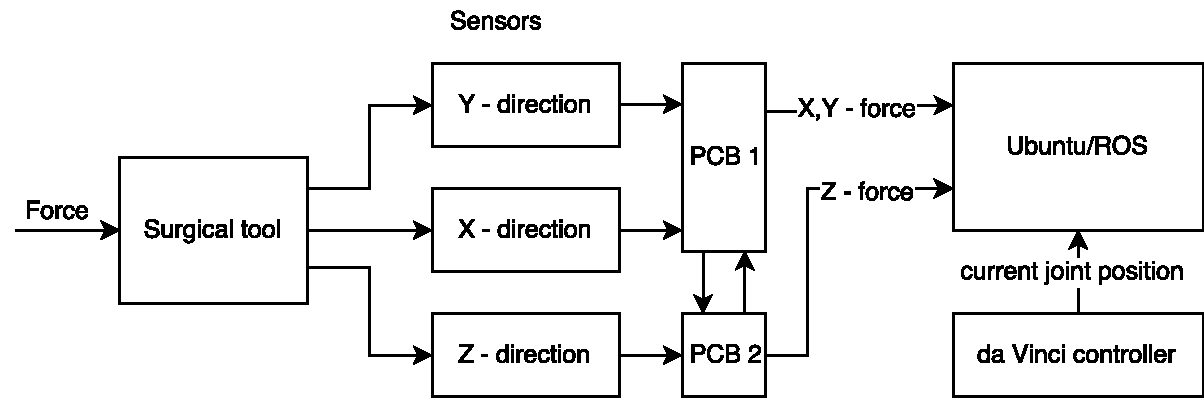
\includegraphics[width=140mm]{fig/methods/dbd2.pdf}
	\end{center}
	\vspace{-4mm}
	\caption[Block diagram]
	{Block diagram}
	\label{fig:BlockDiag}
	\vspace{-2mm}
\end{figure}

\section{Sensor Placement Optimization}
\label{sec:SimMod}
A finite element analysis was done in Solidworks to assess better placement of the strain gauges on the created device. In order to run finite element analysis material properties, such as elastic modulus, poisson`s ratio, and density are necessary to know. Sleeve material is aluminum 6061, that has elastic modulus 68.9 GPa, poisson`s ratio 0.33, and density 2700 kg/m\textsuperscript{3} \cite{aluminum_properties}. Since the shaft and cannula materials are unknown, in order to run finite element analysis their elasticity modulus and density were found experimentally.
	
	\subsection{Elastic Modulus Measurements}
	\label{sec:ElasMod}
	Elastic Modulus of the shaft and the cannula were found experimentally (Figure \ref{fig:ElasModSet}). One end of the observing sample (shaft/cannula) was fixed and the force was applied on the other end. We used weights 250g for the shaft and 555g for the cannula to apply forces. The deformation caused by forces was detected with dial indicator. Experiment was done 5 times, average displacement value was used to calculate elastic modulus. Results are shown in Table \ref{tab:elasMod}.
	
\begin{figure}[h]
	\begin{center}
		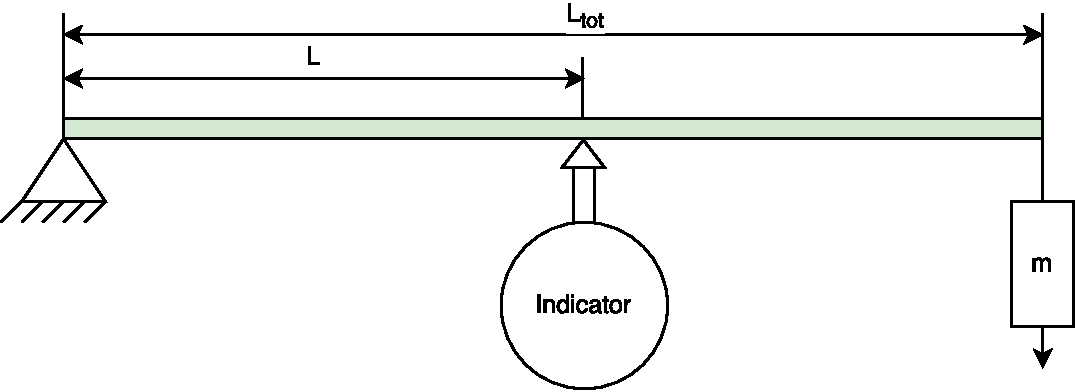
\includegraphics[width=120mm]{fig/methods/el_mod_set.pdf}
	\end{center}
	\vspace{-4mm}
	\caption[Setup to measure elasticity modulus]
	{Setup to measure elasticity modulus}
	\label{fig:ElasModSet}
	\vspace{-2mm}
\end{figure}

\begin{table}
\caption {Elasticity Modulus Measurement Data} \label{tab:elasMod} 
\begin{tabular}{ | c | c | c | c | c | c | c | c | } 
\hline
Component & $d_o$, mm & $d_i$, mm & $I$, mm\textsuperscript{4} & $m$, g & $F$, N & $L$, mm & $L_{tot}$, mm \\ 
\hline
Shaft & 8.4 & 6 & $1.808 \cdot 10^{-10}$ & 250 & 3.25 & 276.2 & 366.8\\ 
\hline
Cannula & 10.54 & 8.75 & $3.181 \cdot 10^{-10}$ & 555 & 6.011 & 95.5 & 105.55 \\ 
\hline
\end{tabular}

\begin{tabular}{ | c | c | c | } 
\hline
Component & $\delta \pm SD$, mm & $E \pm SD$, GPa \\ 
\hline
Shaft & $2.856 \pm 0.123$ & $44.31 \pm 1.86$ \\ 
\hline
Cannula & $0.086 \pm 0.004$ & $63.92 \pm 2.97$ \\ 
\hline
\end{tabular}
\end{table}

Elastic Modulus was found using following equation:

\begin{equation}
E = \frac{FL^3}{3 \delta I} 
\end{equation}

where $F$ - force, $L$ - length from the fixed point to indicator, $I$ - area moment of inertia, $\delta$ - displacement.

Area moment of Inertia: 
\begin{equation}
I = \frac{\pi (d_o^4 - d_i^4)}{64}
\end{equation}

where $d_o$ - cylinder outside diameter, $d_i$- cylinder inside diameter.

Force acting on indicator:
\begin{equation}
F = \frac{L_{tot}}{L}mg
\end{equation}

where $L_{tot}$ - total length of the object, $m$ - mass of the weight, $g$ - gravitational constant.

Experimentally found mean value of elastic modulus of the shaft is equal to 44.31 GPa with standard deviation (SD) 1.86 GPa, elastic modulus of the cannula is 63.92 GPa with SD 2.97 GPa.

	\subsection{Density Measurements}
	\label{sec:DenMeas}
Density was found using following equation:

\begin{equation}
p=\frac{m}{V}
\end{equation}

where $m$ - mass, $V$ - volume.

Weight was measured using mechanical scale. Volume of the shaft was found by following equation: $V =  \pi h(r_o^2-r_i^2) = 4.36 \cdot 10^{-5} m^3$. Volume of the cannula was found using water displacement method. Shaft material density is 473 kg/m\textsuperscript{3}, cannula material density is 55238 kg/m\textsuperscript{3}.

\subsection{Simulation Results}
\label{sec:FEAres}
The mounting location of the active strain gauges should be under the greatest amount of strain. From the Figure \ref{fig:XYdev}, it can be seen that strain gauges for X-Y direction device should be mounted on the area shown green, that corresponds to strain value approximately equal to $1.5 \cdot 10^{-4}$. Passive strain gauges, that will be used only for temperature compensation, will be placed on the blue area perpendicular to the active strain gauges.

\begin{figure}[h]
	\begin{center}
		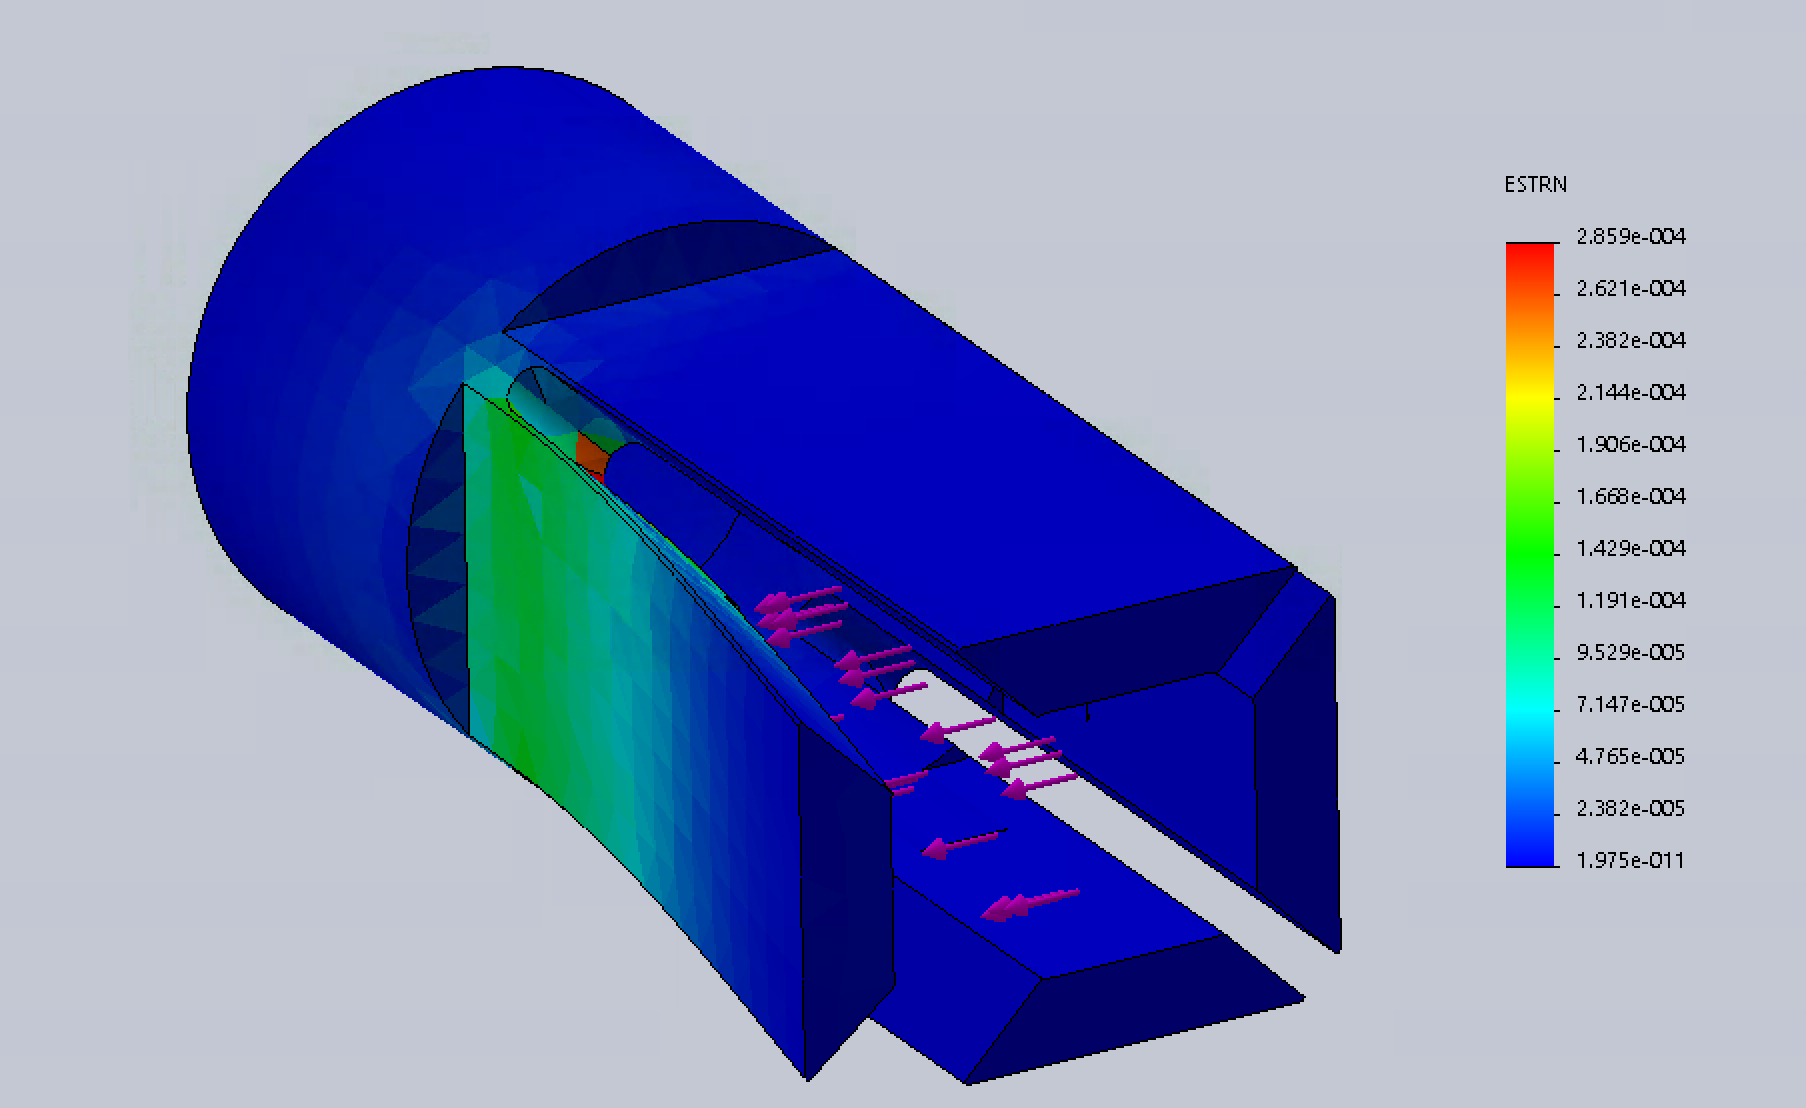
\includegraphics[width=100mm]{fig/methods/old_sleeve.png}
	\end{center}
	\vspace{-4mm}
	\caption[X-Y device]
	{Strain in the device to measure forces in X-Y direction}
	\label{fig:XYdev}
	\vspace{-2mm}
\end{figure}


\begin{figure}[h]
	\begin{center}
		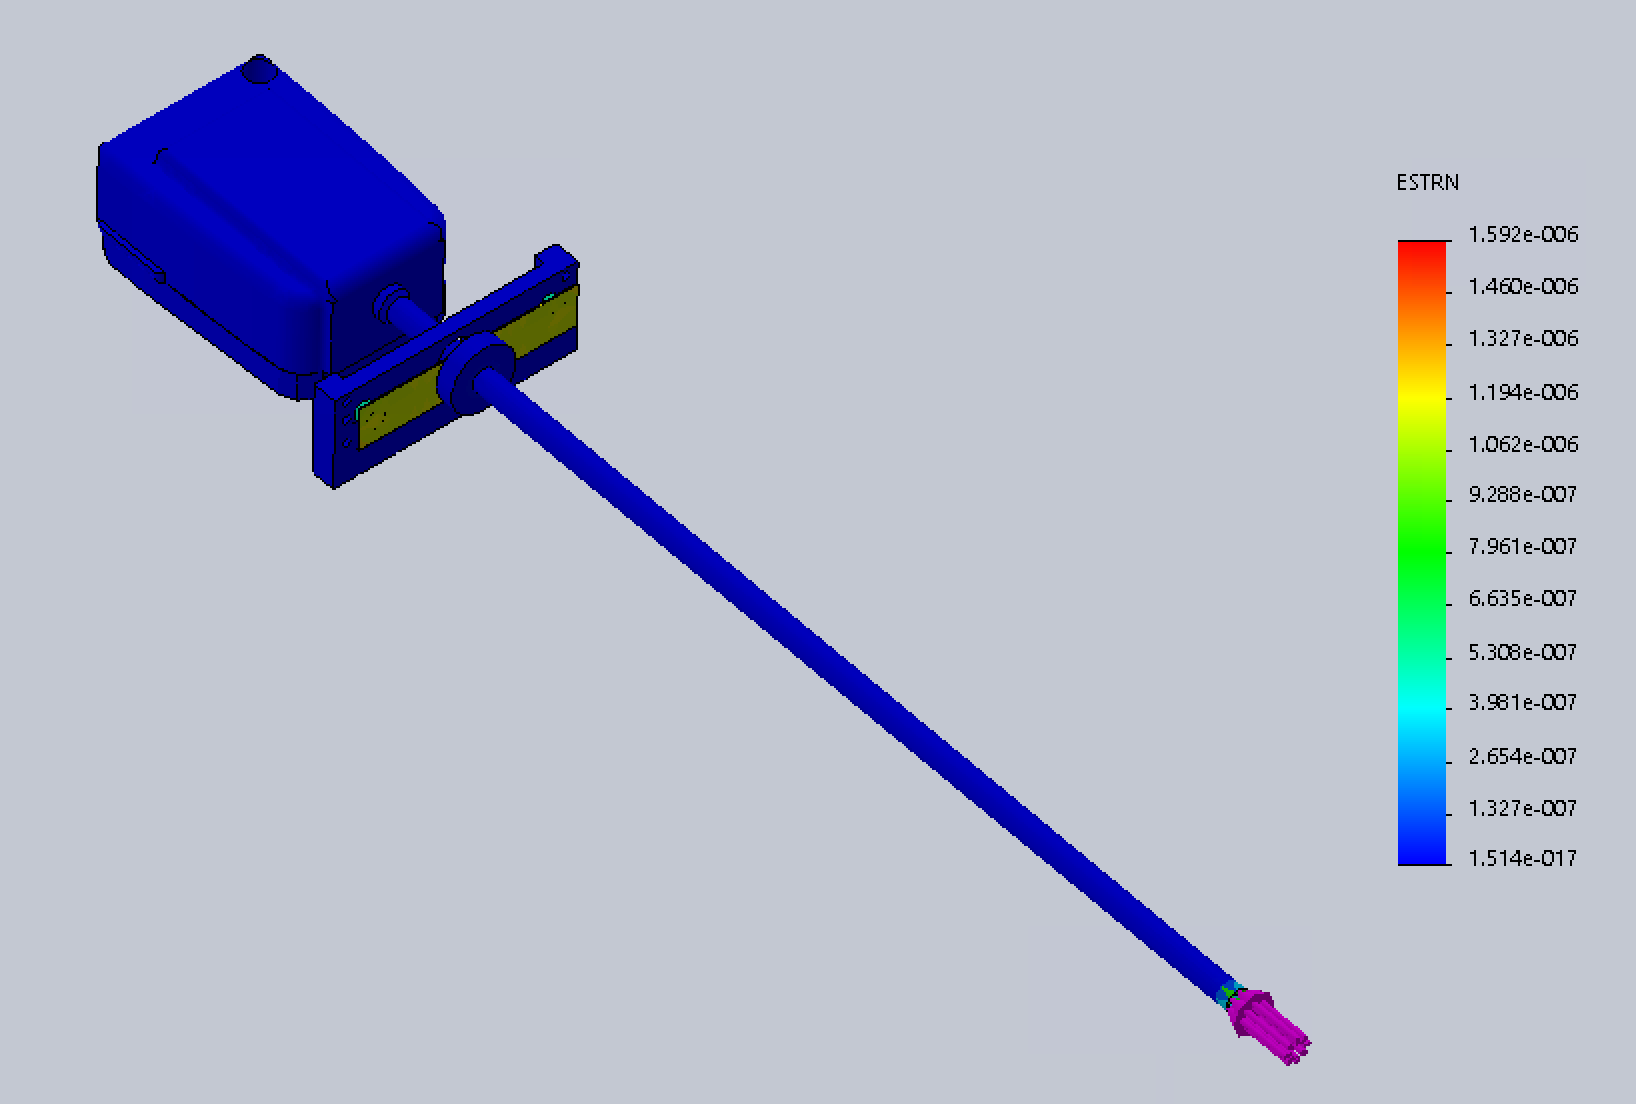
\includegraphics[width=100mm]{fig/methods/z_dir_sim.png}
	\end{center}
	\vspace{-4mm}
	\caption[Z device]
	{Strain in the device to measure forces in Z direction}
	\label{fig:Zdev}
	\vspace{-2mm}
\end{figure}

For Z-direction measurement forces (Figure \ref{fig:Zdev}), area shown with yellow-green color under the highest strain. On both sides and both ends of this plate strain gauges should be placed to form full bridge.

\begin{table}
\caption {Material Properties} \label{tab:matProp} 
\begin{center}
\begin{tabular}{ | c | c | c | c | c | c | c | c | } 
\hline
Component & Elastic Modulus, GPa & Density, kg/ m\textsuperscript{3} \\ 
\hline
Shaft & 44.31 & 473\\ 
\hline
Cannula & 63.92 & 55238 \\ 
\hline
Sleeve & 68.9 & 2700  \\ 
\hline
\end{tabular}
\end{center}
\end{table}

All material properties used for simulations are listed in Table \ref{tab:matProp}.

\section{Requirements for the Device}
	\label{sec:DevReq}
	From the literature review, following requirements for the device were outlined:
	
	Biocompatibility: Z-device is attached to sterile adapter and does not have to be biocompatible. X-Y device goes inside the patient, it means that it should be sterilized and created using biocompatible materials. Current version of the device is not biocompatible. We can achieve biocompatibilty by using Stainless Steel as a device material and biocompatible epoxy to cover strain gauges, also teflon coated wires should be used for all electrical connections.
	
	Force range: Some studies \cite{mack_interactive_2012, prasad_modular_2003, } have shown that force range applied during surgeries lies in range (0-11 N). The designed device measures forces in that range, and if the force goes beyond that range it can be used to trigger safety alert.
	
	Force sensitivity: The device should be sensitive enough with minimum detectable signal (MDS) at least 0.3 N and give accurate readings (error < 0.05 N) \cite{mack_interactive_2012}.
	
	Speed of force reading: Device is used for real-time haptic feedback, the minimum requirement for data acquisition speed is 500 Hz. The created device is compliant with mentioned requirements.
	
	No restriction of motion range of the device: We were able to measure force in three directions independently from each other using separate wheatstone bridges for each direction. At the same time tool can rotate freely and change depth of insertion.	
	
	Linearity: Strain gauges have linear response with deformation. Our calibration results have shown linearity of the readings.

	Device modularity: Force-sensing devices were designed to fit daVinci cannula and sterile adapter and compensate tolerances by adjustment of set screws.
	
\section{Mechanical Design}
\label{sec:mechDes}

	\subsection{Strain Gauge}
	\label{sec:SGReq}
	According to the manual for strain gauge selection provided by Vishay Micro-Measurements, the strain gauge should have following parameters:
\begin{itemize}
  \item Single grid for unidirectional force measurements;
  \item Isoelastic (D alloy) that has higher gauge factor with E backing;
  \item Encapsulated with pre attached leads for easier placement;
  \item STC (self-temperature-compensation) - small temperature dependence;
\end{itemize}	
	
Maximum strain on the created device is $1.5 \cdot 10^{-4}$, in case of 10 N load with maximally opened shaft. From the literature, strain gauges length should be more than 5\% of maximum strain, hence, minimum length of the strain gauge should be 0.0075 mm. 

Gauge Factor (GF) for strain gauges usually is 2. According to the formula (\ref{eq:resistance}) strain gauge with resistance 120 $\Omega$ have maximum change in resistance equal to 0.036 $\Omega$, and 350  - 0.105 $\Omega$:

\begin{equation}\label{eq:resistance}
\Delta R=GF \cdot R \cdot \varepsilon
\end{equation}

where $GF$ - gauge factor, $R$ - resistance, $\varepsilon$- strain.

For the device strain gauges with resistance 350 $\Omega$, GF is 2, single grid, encapsulated with pre-attached leads were used.

	\subsection{Installation of Strain Gauges}
	\label{sec:instSG}

	Application of strain gauges was done following the manual provided by Vishay Micro-Measurements. \cite{StrGugeInst}.

	First the working surface (glass) and tweezers were cleaned with Neutralizer 5. After that shaft surface preparation was started, using solvent degreaser GC-6 Isopropyl Alcohol. A gauge layout was then applied with a 4H drafting pencil. The surface was then conditioned with Conditioner A and the extra liquid was wiped with gauze. Finally, the surface was then neutralized with M-Prep Neutralizer 5A. \cite{StrGugeInst}

	The strain gauges were first placed on the glass and then transported using mylar tape onto the instrument surface. A thin layer of catalyst was applied on the strain gauge and given one minute to dry. Then adhesive M-BOND 200 was applied on the surface, pressure was applied on the tape for one minute, then two more minutes to let it dry before the tape was removed. Then leads soldering was done by application of pats, and soldering them with thin wires. \cite{youtube}

	The methodology of the strain gauge application more specifically described in \cite{StrGugeInst}.

	In compliance with the literature \cite{StrGugeInst} for application of the strain gauge on metals, the same materials and technique can be used. Therefore, the same method was used to apply strain gauges on different materials.

\subsection{X-Y direction}
\label{sec:xyDir}

XY-device consists of one sleeve and one set screw. We manufactured sleeve using Aluminum 6061 Alloy. %First, hole with diameter 9.5 mm should be drilled in the center using the lathe machine. Then on the milling machine all the side slots and inner square should be milled. On the same machine hole for the set screw should be drilled. After that set screw thread was tapped.%
The manufactured sleeve is placed on the cannula end and is fixed with a set screw on the top.

\begin{figure}[h]
	\begin{center}
		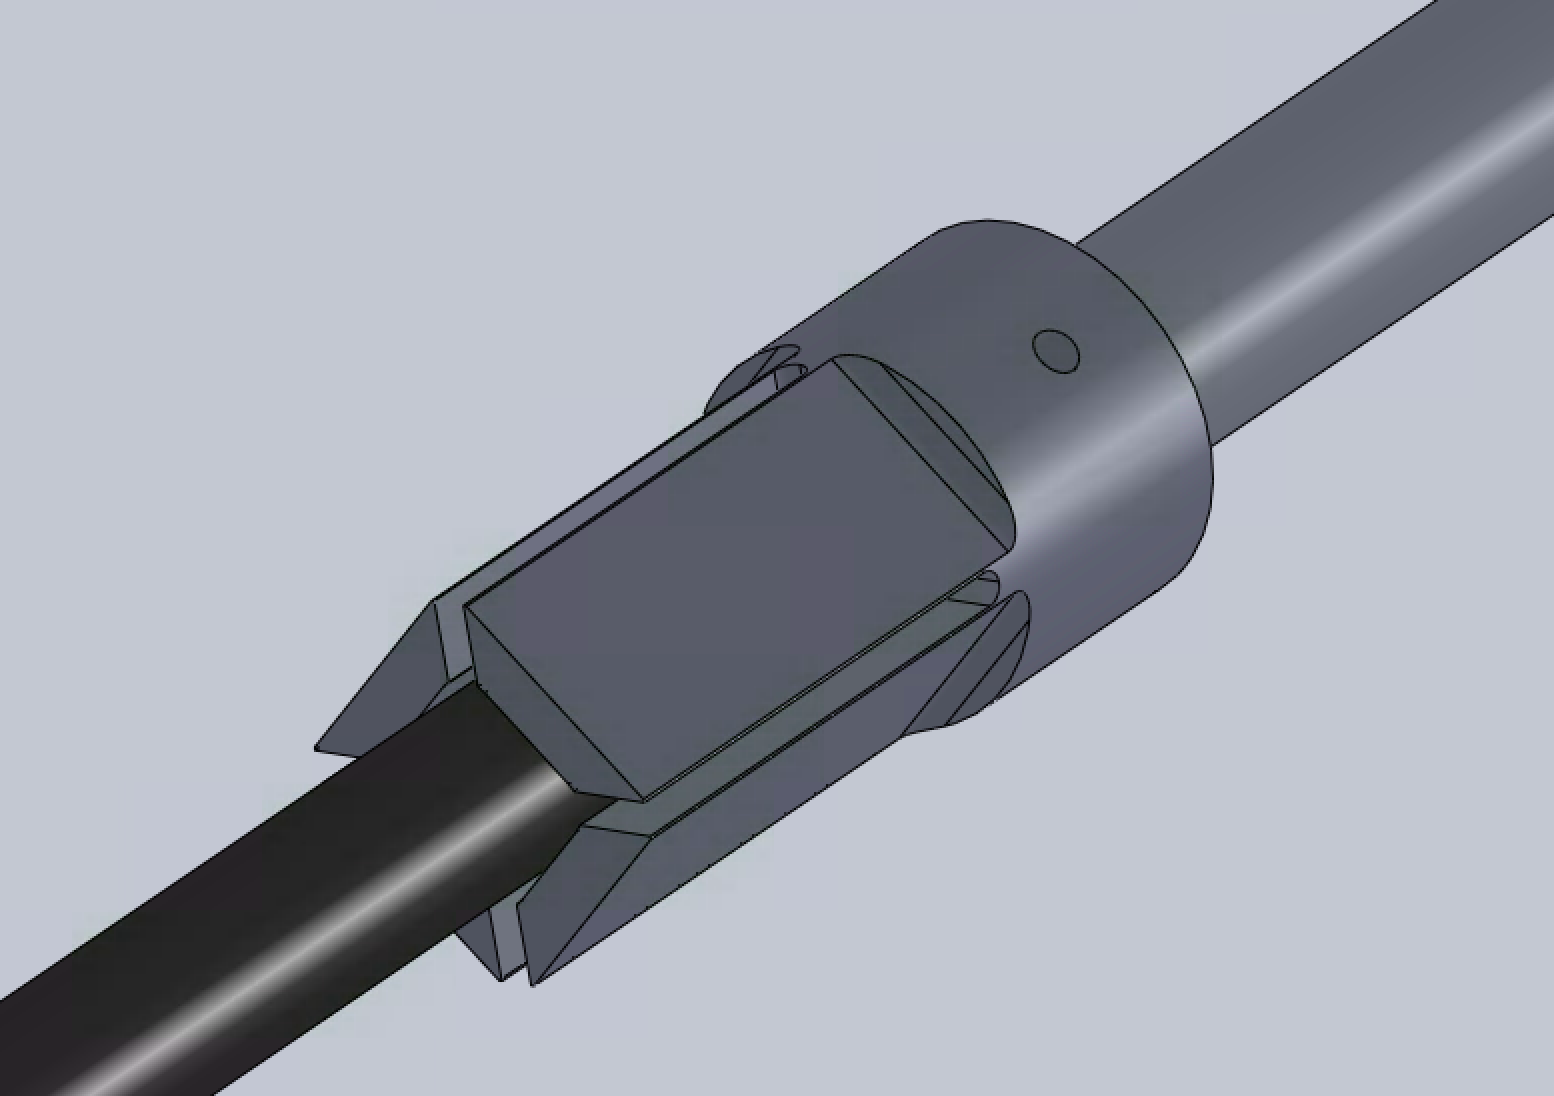
\includegraphics[width=80mm]{fig/methods/xy_dev_cl.png}
	\end{center}
	\vspace{-4mm}
	\caption[XY-direction force feedback sensor]
	{XY-direction force feedback sensor}
	\label{fig:xy-direction}
	\vspace{-2mm}
\end{figure}

\begin{figure}[h]
	\begin{center}
		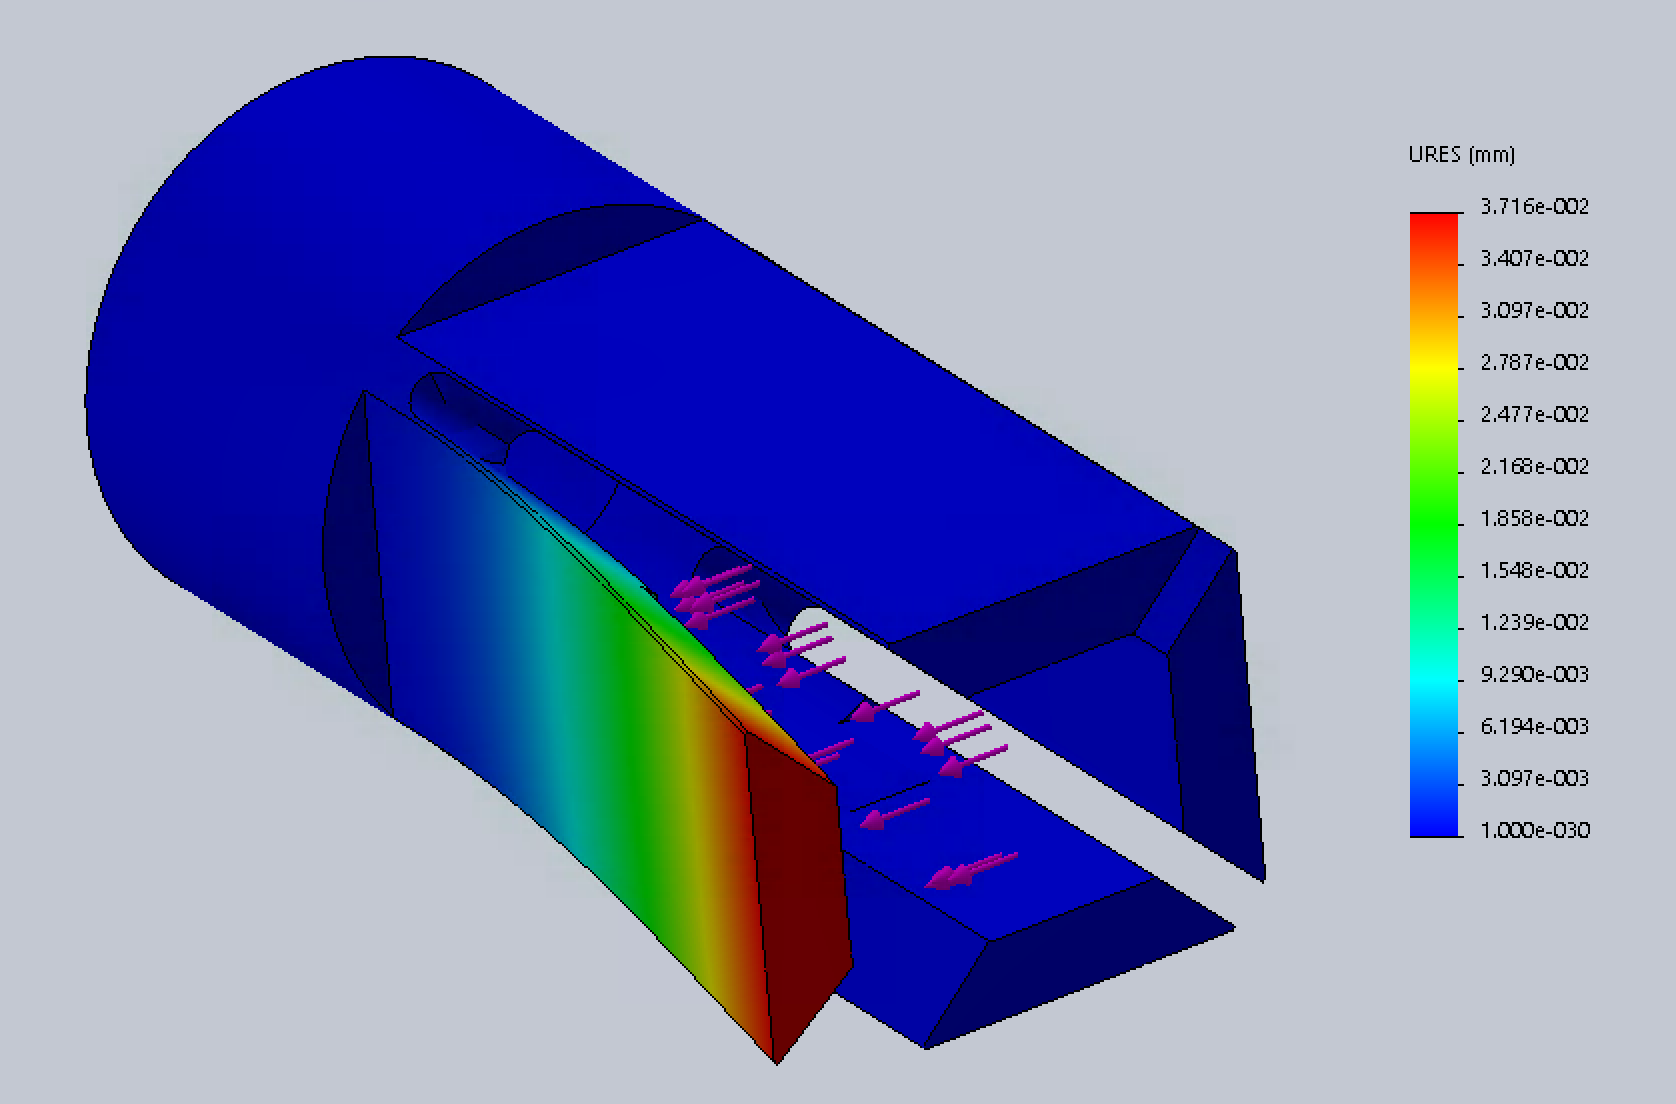
\includegraphics[width=80mm]{fig/methods/old_sleeve_displ.png}
	\end{center}
	\vspace{-4mm}
	\caption[XY-direction force feedback sensor]
	{Displacement of XY device}
	\label{fig:xy-displ}
	\vspace{-2mm}
\end{figure}

In order to get accurate readings maximum displacement of the sleeve sides should prevent shaft from hitting the cannula. It means that it should be less than $d=(d_{can_in} - d_{shaft_out})/2 = (8.75 - 8.4)/2 = 0.175$ mm. From the Solidworks simulation (Figure \ref{fig:xy-displ}), maximum displacement is 0.037 mm, which is in appropriate range.

\subsection{Z-direction}
\label{sec:zDir}

\begin{figure}[h]
	\begin{center}
		\includegraphics[width=80mm]{fig/methods/z_dir_design.png}
	\end{center}
	\vspace{-4mm}
	\caption[Z-direction force feedback sensor]
	{Z-direction force feedback sensor}
	\label{fig:Z-direction}
	\vspace{-2mm}
\end{figure}

\begin{figure}[h]
	\begin{center}
		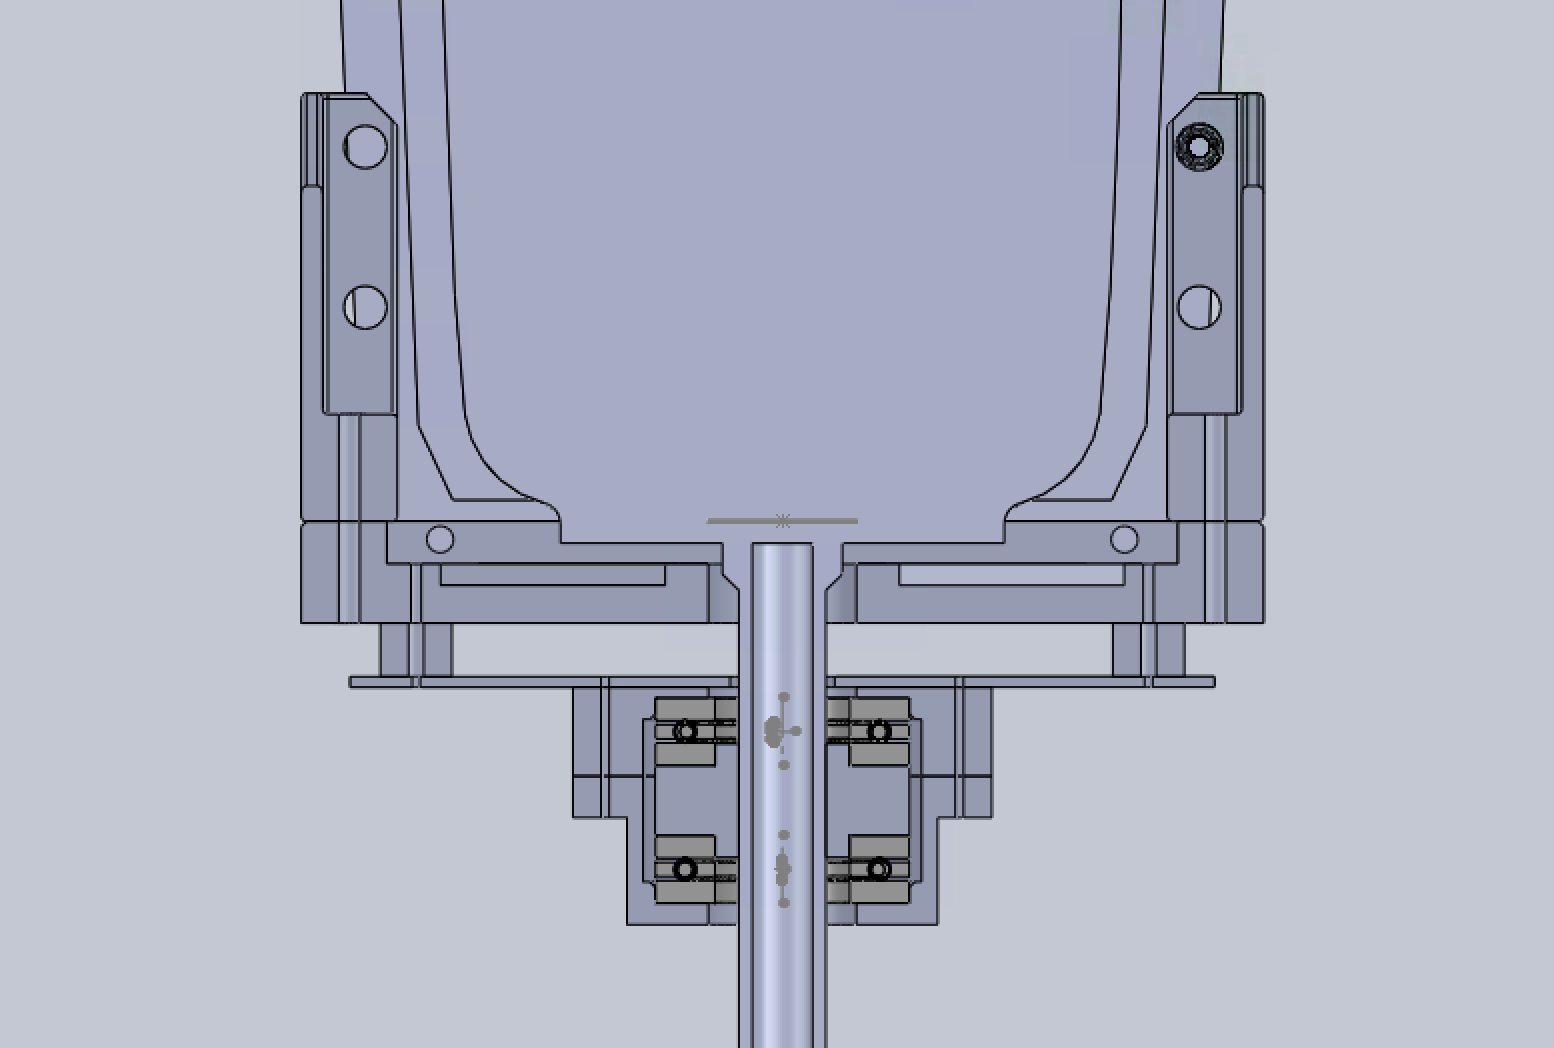
\includegraphics[width=80mm]{fig/methods/z_dir_sec.png}
	\end{center}
	\vspace{-4mm}
	\caption[Z-direction force feedback sensor - section vew]
	{Z-direction force feedback sensor - section vew}
	\label{fig:Z-direction_sec}
	\vspace{-2mm}
\end{figure}


Z-device (Figures \ref{fig:Z-direction}, \ref{fig:Z-direction_sec}) consists of attachment to the sterile adapter, 2 thrust ball bearings, three rings, plate, and two cylindrical spacers. Three rings and two ball bearings are used to transfer only z-directional forces further to the plate and keep ability of the shaft to rotate. The ring in the center is in direct contact with the instrument shaft, two outer rings are for the push and pull forces transfer. The plate experience maximum strain and all strain gauge sensors are mounted on it.  Two cylindrical spacers are used to give plate space to move and they are mounted on the attachment plate. the attachment plate consist of three plates, they are press fitted on the sterile adapter and fixed with four set screws.

Three rings and plate were manufactured with Aluminum Alloy 6061, attachment parts were 3-D printed, fasteners were used as spacers.


\section{Electrical and Software Design}
\label{sec:elecDes}

	\subsection{Circuit design}
	\label{sec:cirDes}
	Block diagram of the PCB is shown on Figure \ref{fig:PCB_block_diag}. 

\begin{figure}[h]
	\begin{center}
		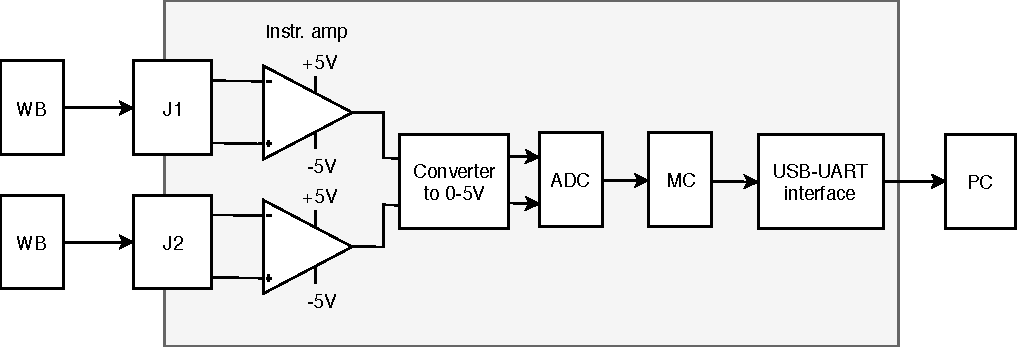
\includegraphics[width=140mm]{fig/methods/PCB_diagram.pdf}
	\end{center}
	\vspace{-4mm}
	\caption[Block diagram of the circuit]
	{Block diagram of the circuit}
	\label{fig:PCB_block_diag}
	\vspace{-2mm}
\end{figure}
	
\begin{figure}[h]
	\begin{center}
		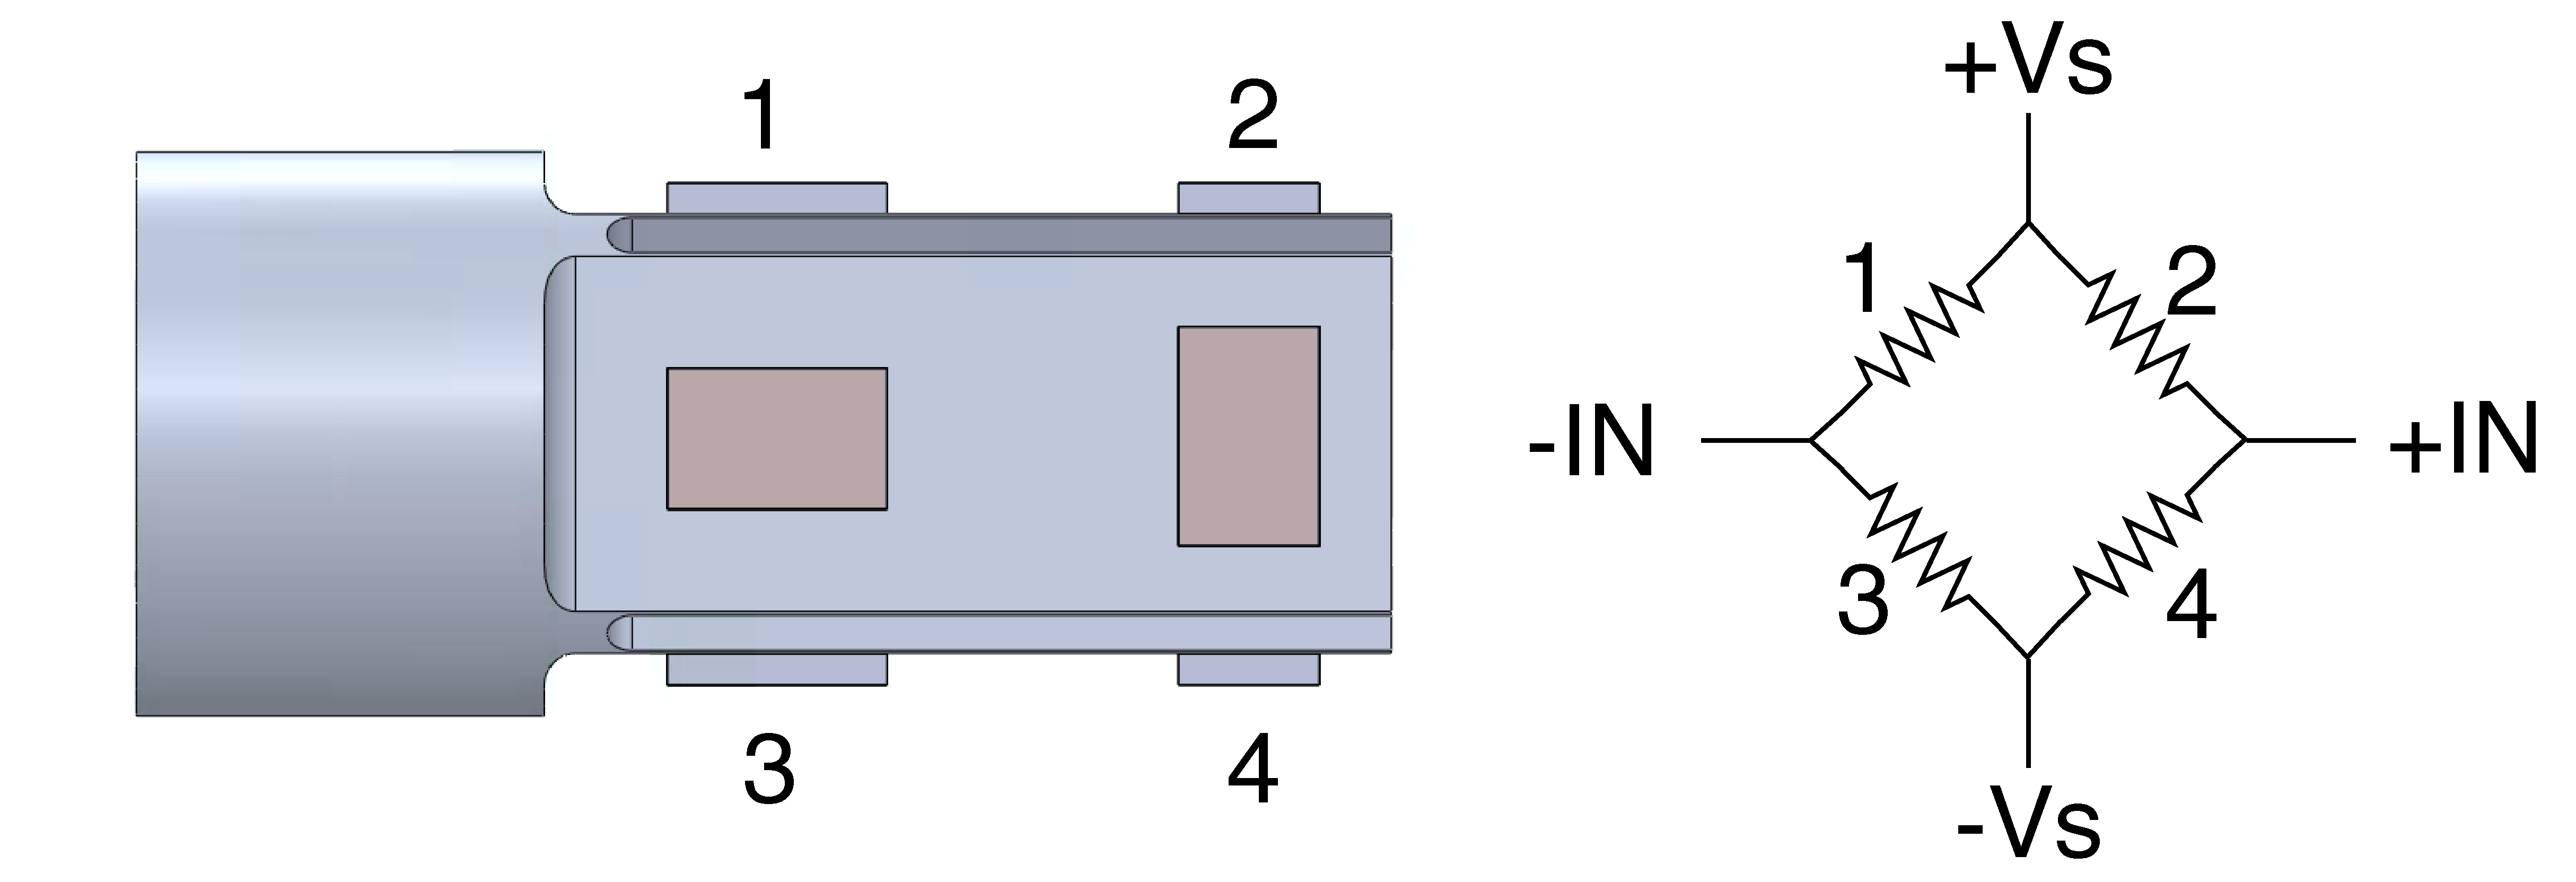
\includegraphics[width=120mm]{fig/methods/Wiring_xy_sleeve.pdf}
	\end{center}
	\vspace{-4mm}
	\caption[Wheatstone bridge configuration of XY-device]
	{Wheatstone bridge configuration of XY-device}
	\label{fig:WB_xy_dev}
	\vspace{-2mm}
\end{figure}

\begin{figure}[h]
	\begin{center}
		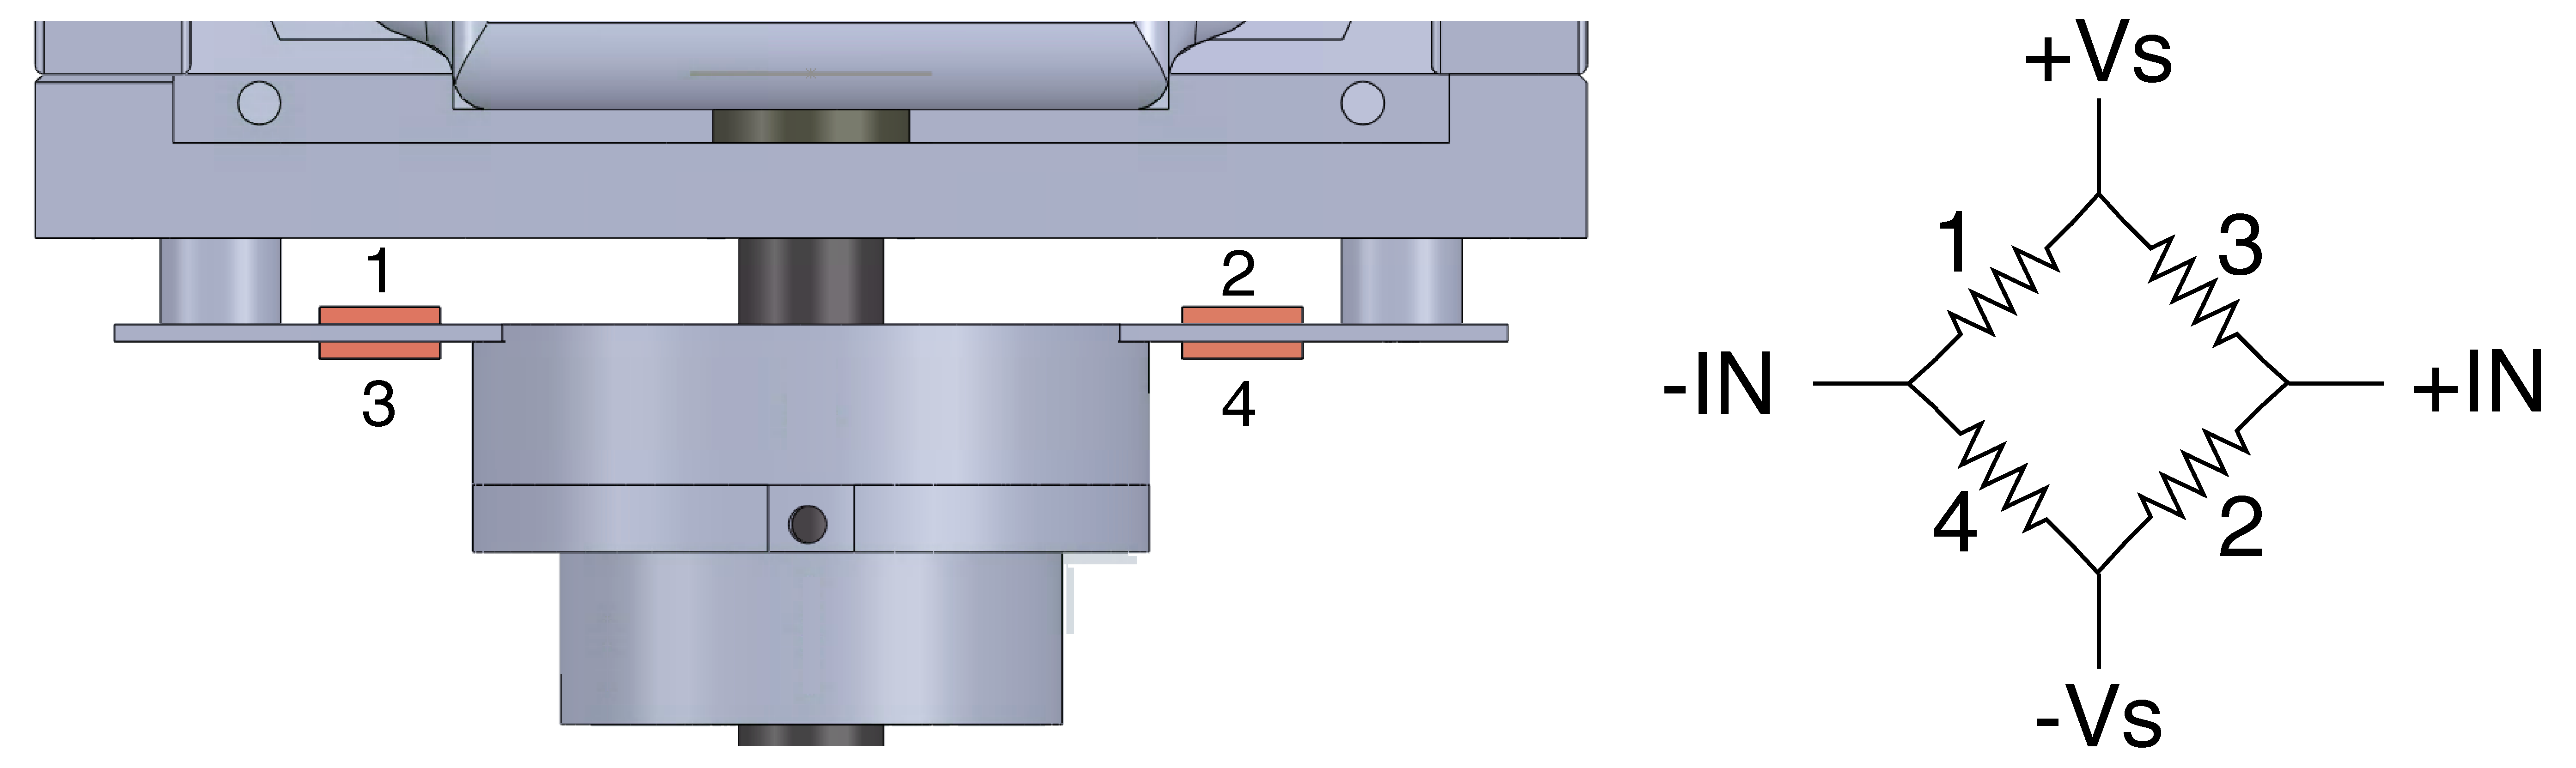
\includegraphics[width=140mm]{fig/methods/Wiring_z.pdf}
	\end{center}
	\vspace{-4mm}
	\caption[Wheatstone bridge configuration of Z-device]
	{Wheatstone bridge configuration of Z-device}
	\label{fig:WB_z}
	\vspace{-2mm}
\end{figure}
	
	Strain gauges are shown with numbers 1-4.
	Using Altium Designer 15.1 PCB was developed and manufactured elsewhere. 

Write about how to calibrate the PCB itself and how it works.

	\subsection{Noise Analysis}
	\label{sec:NoiseExp}
	Noise analysis was performed using oscilloscope ... Make FFT analysis

		\begin{figure}[h]
			\begin{center}
			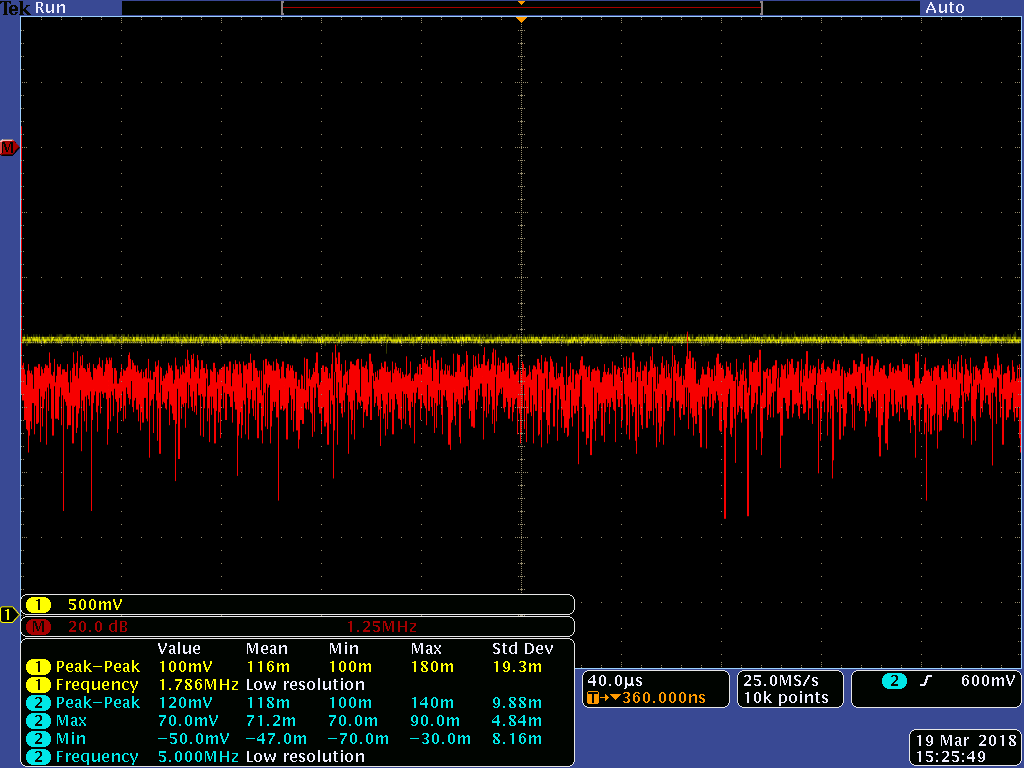
\includegraphics[width=120mm]{fig/results/40us_1stADC.png}
			\end{center}
			\vspace{-4mm}
		\caption[Noise analysis of the output signal]
		{Noise analysis of the output signal}
		\label{fig:OutputSignal}
		\vspace{-2mm}
		\end{figure}

	\subsection{Microcontroller Software}
	\label{sec:MicrSoft}
	We use arduino for ..
	Filtering was implemented on microcontroller by finding average of recent 5 readings 
	Filtering - ideally small time delay. Total teleoperation cycle delay - less than 100ms (visually noticeable delay). Kalman filter? Use same parameters for both signals to get identical time delay.
	good article about changing baud rate.

	\subsection{ROS Architecture}
	\label{sec:p2}
	
\section{Calibration}
\label{section:Calibration}
First we used set of weights applied in two directions, but since the system was too sensitive for direction of force, we had to change our approach of determining the force direction. It was decided to use optical tracking system for that purpose.

	\subsection{Calibration Setup}
	\label{sec:CalSetup}
	Tell how calibration with optical tracking system is working

	\subsection{Calibration of the Load Cell}
	\label{sec:CalLoadCell}
	Was pefrormed using following setup cite figure ..
	Calibration equation we got ..

	\subsection{Calibration Results}
	Find mean square root error

		\begin{figure}
			\centering
			\begin{subfigure}
				\centering
				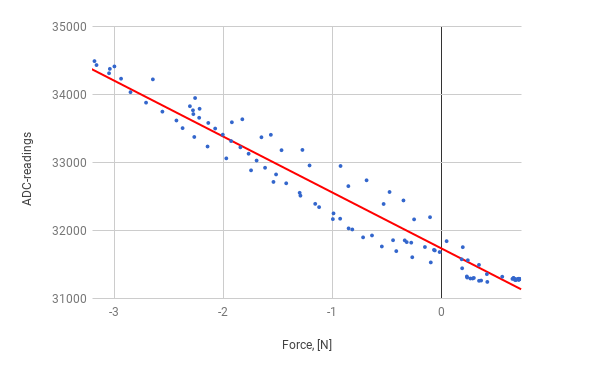
\includegraphics[width=120mm]{fig/results/x-dir.png}
				\caption{X-component}
				\label{fig:Xdirection}
			\end{subfigure}
			\begin{subfigure}
				\centering
				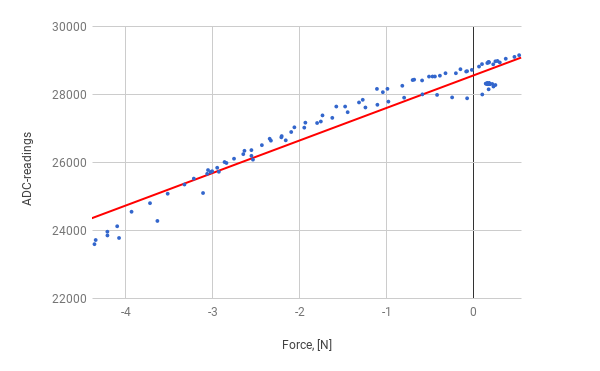
\includegraphics[width=120mm]{fig/results/y-dir.png}
				\caption{Y-component}
				\label{fig:Ydirection}
			\end{subfigure}
			\caption{Calibration results}
			\label{fig:Calibration}
		\end{figure}
Precision represents capacity of a sensing system to give the same reading when repetitively measuring the same measurand under the same conditions. The precision is a statistical parameter and can be assessed by the standard deviation (or variance) of a set of readings of the system for similar inputs.

One of the measurements of signal quality is signal-to-noise ratio (SNR). A higher value of SNR means the clear acquisitions with low signal distortions and artifacts caused by unwanted noise. It is defined as:

\begin{equation}
\frac{S}{N}=\frac{Mean value of signal}{Standard deviation of noise}
\end{equation}

For X-direction SNR is $3232 \pm 78$, for Y-direction SNR is $2857 \pm 150$, which is much bigger than 1. It means that system has very low noise.

Error is the difference between the actual value of the measurand and the value produced by the sensing system. Error can be caused by a variety of internal and external sources and is closely related to accuracy. Accuracy can be related to absolute or relative error as:

\begin{equation}
Absolute error = \frac{Output}{ True value}
\end{equation}

From figure we can assume that fluctuations in the output signal are due to systematic errors. 

Drift is observed when a gradual change in the sensing system’s output is seen, while the measurand actually remains constant. Drift is the undesired change that is unrelated to the measurand. It is considered a systematic error, which can be attributed to interfering parameters such as mechanical instability and temperature instability, contamination, and the sensor’s materials degradation. 

Resolution (or discrimination) is the minimal change of the measurand that can produce a detectable increment in the output signal. Resolution is strongly limited by any noise in the signal.

In a sensing system, minimum detectable signal (MDS) is the minimum signal increment that can be observed, when all interfering factors are taken into account. When the increment is assessed from zero, the value is generally referred to as threshold or detection limit. If the interferences are large relative to the input, it will be difficult to extract a clear signal and a small MDS cannot be obtained.

Sensitivity is the ratio of the incremental change in the sensor’s output (Dy) to the incremental change of the measurand in input (Dx). The slope of the calibration curve, y f(x), can be used for the calculation of sensitivity.

The closeness of the calibration curve to a specified straight line shows the linearity of a sensor. Its degree of resemblance to a straight line describes how linear a system is.

Hysteresis is the difference between output readings for the same measurand, depending on the trajectory followed by the sensor.

The maximum and minimum values of the measurand that can be measured with a sensing system are called the measurement range, which is also called the dynamic range or span. This range results in a meaningful and accurate output for the sensing system. \cite{kalantar-zadeh_sensors_2013}

\section{Experiments}
\label{sec:Experims}

	\subsection{Distance from the cannula to the tip dependence from readings}
	\label{sec:DisExp}
	Distance from the cannula to the tip - measure - 3 ¼ inch. Maximum distance is 9 inches.


	\subsection{Temeperature Dependence}
	\label{sec:TempExp}
	Try in 36.6 Celsius and room temperature
	Effect of the surrounding temperature on the device was ..

	Do all experiments at least three times and calculate all statistic things you can (SD)

	\subsection{Hysteresis}
	\label{sec:HystExp}
	Hysteresis was checked .. 
	We written separate program to check hysteresis





